\begin{figure}[t]
\centering
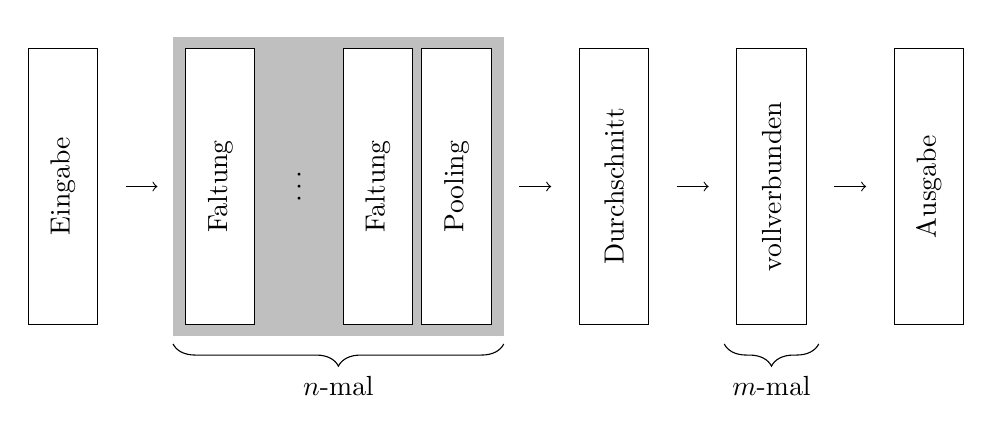
\begin{tikzpicture}
  \tikzstyle{node}=[rectangle,draw, minimum width=100pt, minimum height=25pt, inner sep=0pt, fill=white, rotate=90]
  \tikzstyle{noborder}=[draw=none,fill=none]
  \tikzstyle{color1}=[fill=orange]
  \tikzstyle{path}=[->, shorten >= 10pt, shorten <= 10pt]

  \fill [lightgray] (1.4, -1.9) rectangle (5.6, 1.9) node {};

  \node[node] (0)  at (0, 0) {Eingabe};
  \node[node] (1)  at (2, 0) {Faltung};
  \node[node,noborder] (2)  at (3, 0) {$\ldots$};
  \node[node] (3)  at (4, 0) {Faltung};
  \node[node] (4)  at (5, 0) {Pooling};
  \node[node] (5)  at (7, 0) {Durchschnitt};
  \node[node] (6)  at (9, 0) {vollverbunden};
  \node[node] (7)  at (11, 0) {Ausgabe};

  \path[path] (0) edge (1);
  \path[path] (4) edge (5);
  \path[path] (5) edge (6);
  \path[path] (6) edge (7);

  \draw [decoration={brace,mirror,amplitude=8pt},decorate,-] (1.4,-2) -- node[below=8pt] {$n$-mal} (5.6,-2);
  \draw [decoration={brace,mirror,amplitude=8pt},decorate,-] (8.4,-2) -- node[below=8pt] {$m$-mal} (9.6,-2);
\end{tikzpicture}
\caption[Spektrale Netzarchitektur auf Graphen]{Typische spektrale Netzarchitektur auf Graphen bestehend aus beliebig vielen verketteten Faltungsschichten gefolgt von jeweils einer Poolingschicht.
Im Anschluss sorgt die Benutzung einer Durchschnittsschicht über den Knoten jedes Merkmals für die Verwendung von vollverbundenen Schichten hinzu zur Ausgabe.}
\label{fig:netzarchitektur_spectal}
\end{figure}
